\documentclass[a4paper,10pt]{article}
\usepackage[utf8]{inputenc}
\usepackage{graphicx}
\usepackage[german]{babel}

%opening
\title{Tracing Aufg 11.2}
\author{Can Nayci, Leonhard Rattmann, Emil Sharaf}

\begin{document}

\maketitle

Randnotiz: Die Ausführung des Programms mit Score-P sorgt für Probleme, wie u.a. auch schon bei GS 3/2 (Ende) zu sehen. Daher wurden für die restliche Analyse die Traces von Patricks Gruppe geliehen.

\section{Startphase}
Auf den Ausschnitten ist nicht abgebildet, wie die Verschiedenen Prozesse zu unterschiedlichen Zeiten \textit{MPI\_Init} starten. Womöglich liegt das an dem Hyperthreading; die ersten zwei Prozesse lägen dabei auf z.B. HW-Core 0 usw..\\

Bei GS 3/2 sieht man klar, wie $p_0$ zuerst seine Berechnung macht, $p_1$ damit freigibt usw., also das Treppenmodell ähnlich dem Konzept. Da JA 3/2 paralleler laufen kann und die \textit{Ssend} von $p_0:2$ nicht auf $p_1:1$ warten muss, wie im „Stufenmodell“, sind die \textit{Recv} und \textit{Ssend}-Phasen deutlich kürzer. Der größte Teil bei Jacobi ist also der Rechnungsteil, bei GS die Kommunikation \\

Im anderen Modell wird nach \textit{MPI\_Init} erst das options-struct per Broadcast verschickt (da askParams() bei allen Prozessen läuft ist das optional). Da diese Operation bei allen Methoden gleich ist, sieht man ein ähnliches fast-dreieckiges Muster um den Broadcast. In beiden Jacobi-Läufen fangen die Recheniterationen zeitversetzt an; ebenso bei GS. Das Springen in die nächste Iteration bei GS hängt bei beiden Läufen v.a. am Warten auf die Haloline, bei Jacobi beim Austauschen des Residuums und dem Senden der Haloline.\\
\begin{figure}[h!]
  \caption{Startphase GS 3/2}
  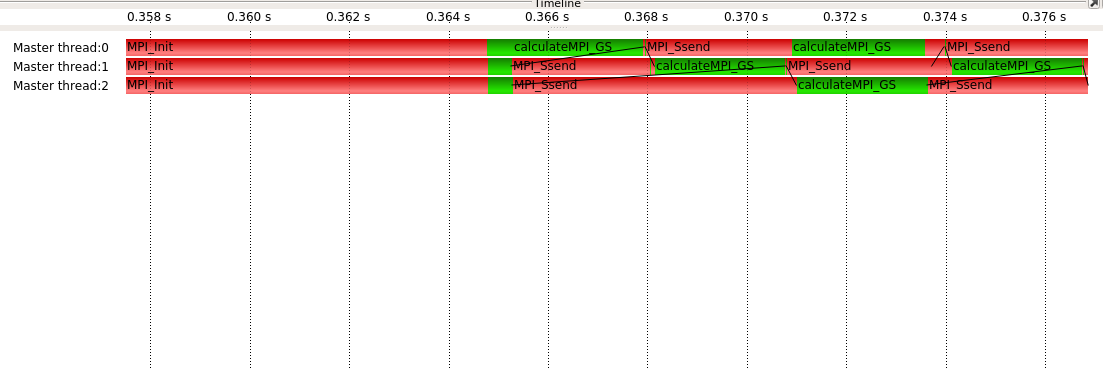
\includegraphics[width=14cm]{c_start_GS_3x2.png}
\end{figure}

\begin{figure}[h!]
  \caption{Startphase GS 3/2 (Patrick)}
  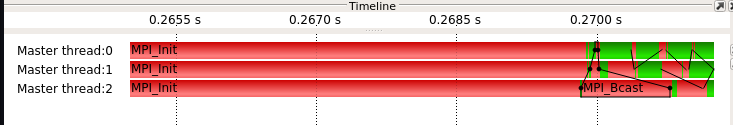
\includegraphics[width=14cm]{Patrick/c_start_GS_3x2.png}
\end{figure}
\begin{figure}[h!]
  \caption{Startphase GS 5/4 (Patrick)}
  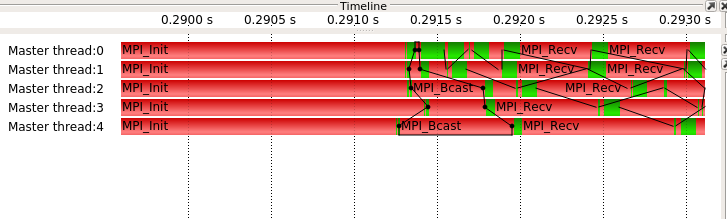
\includegraphics[width=14cm]{Patrick/c_start_GS_5x4.png}
\end{figure}
\begin{figure}[h!]
  \caption{Startphase JA 3/2}
  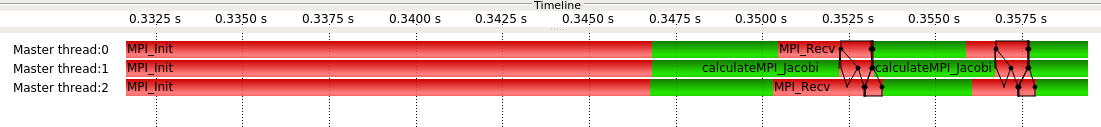
\includegraphics[width=14cm]{c_start_JA_3x2.png}
\end{figure}
\begin{figure}[h!]
  \caption{Startphase JA 3/2 (Patrick)}
  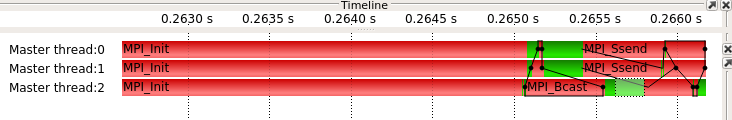
\includegraphics[width=14cm]{Patrick/c_start_JA_3x2.png}
\end{figure}
\begin{figure}[h!]
  \caption{Startphase JA 5/4 (Patrick)}
  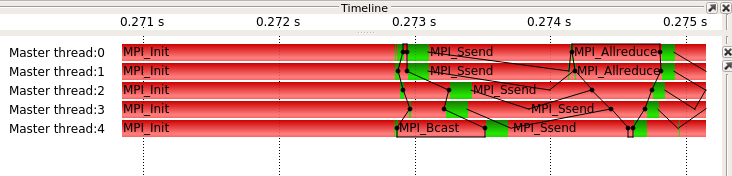
\includegraphics[width=14cm]{Patrick/c_start_JA_5x4.png}
\end{figure}


\section{Synchronisation}
Zur Synchronisation haben alle Varianten des Codes verschiede Ansätze: Bei unserem JA tauschen sich die Hälfte der Prozesse gleichzeitig aus, bei GS tauschen sie die Halolines aus, wenn sie benötigt werden. Beim anderen Modell werden die Daten in JA sequentialisiert ausgetauscht, in GS ähnlich wie bei uns, mit \textit{Issend} statt \textit{Ssend}. Bei allen Herangehensweisen sieht man die kurzen grünen Abschnitte, bei denen die calculate()-Methode die Kommunikation aufruft und danach darauf wartet.\\

Bei unserem Modell ist ersichtlich, dass Berechnungen in GS teilweise parallel stattfinden, allerdings klar in Abhängigkeit voneinander, also stufend. In Patricks Ansatz, gerade bei 5/4 sieht man eine freiere Positionierung der Rechenphasen.\\

Bei JA sieht man die sequentielle und parallele Kommunikation der verschiedenen Modelle, da in JA 5/4 wieder Stufen zu sehen sind (gerade bei Allreduce).

\begin{figure}[h!]
 \caption{Synchronisation GS 3/2}
 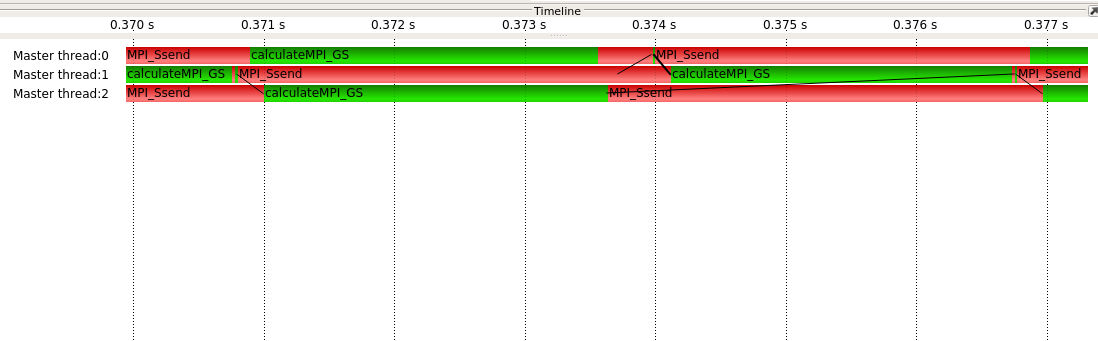
\includegraphics[width=14cm]{c_sync_GS_3x2.png}
\end{figure}

\begin{figure}[h!]
 \caption{Synchronisation GS 3/2 (Patrick)}
 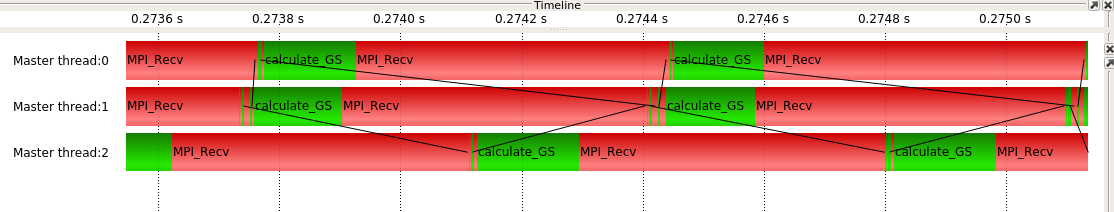
\includegraphics[width=14cm]{Patrick/c_sync_GS_3x2.png}
\end{figure}
\begin{figure}[h!]
 \caption{Synchronisation GS 5/4 (Patrick)}
 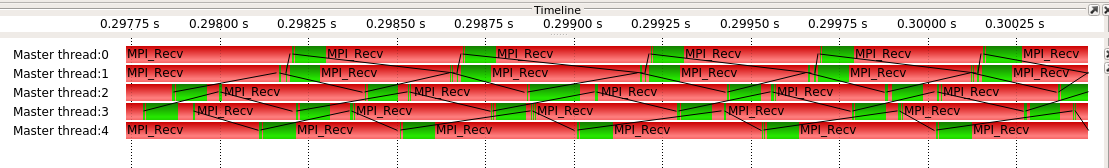
\includegraphics[width=14cm]{Patrick/c_sync_GS_5x4.png}
\end{figure}
\begin{figure}[h!]
 \caption{Synchronisation JA 3/2}
 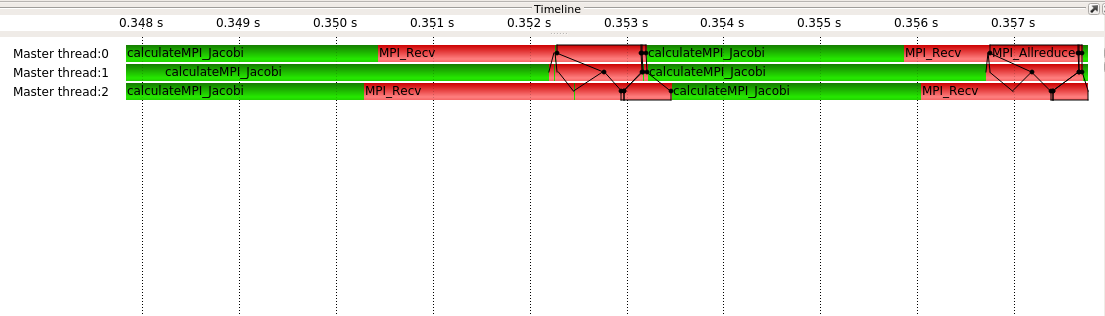
\includegraphics[width=14cm]{c_sync_JA_3x2.png}
\end{figure}
\begin{figure}[h!]
 \caption{Synchronisation JA 3/2 (Patrick)}
 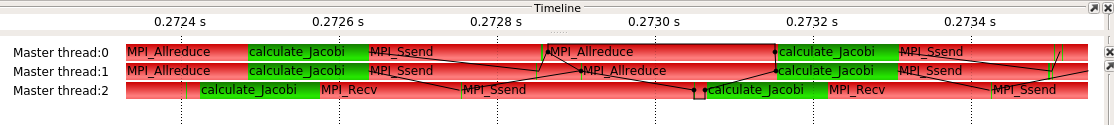
\includegraphics[width=14cm]{Patrick/c_sync_JA_3x2.png}
\end{figure}
\begin{figure}[h!]
 \caption{Synchronisation JA 5/4 (Patrick)}
 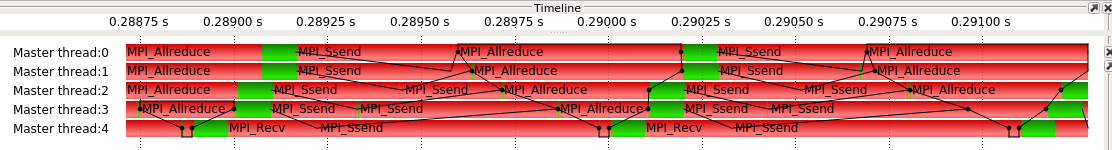
\includegraphics[width=14cm]{Patrick/c_sync_JA_5x4.png}
\end{figure}

\section{Endphase}
Bei der Endphase sieht man bei unseren GS 3/2 offensichtlich, dass \textit{MPI\_Finalize} nicht stattfindet, evtl. wg nicht gesäuberten Issends. Da hier aber nicht einmal displayMatrix() angezeigt wird (aber definitiv ausgeführt wird), ist es wahrscheinlicher, dass die Spurdaten verfälscht sind.\\

Die DisplayMatrix()-Kommunikation ist bei allen Modellen wieder identisch. Bei GS 5/4 sieht man interessanterweise eine Kreuzung der Sendungen, allerdings nicht bei JA 5/4. Eventuell gibt es hier einen Zusammenhang zwischen der \textit{MPI\_Finalize}-Zeit, die bei GS deutlich unregelmäßiger ist als bei JA (auch mit den verschiedenen Skalierungen).
\begin{figure}[h!]
 \caption{Endphase GS 3/2}
 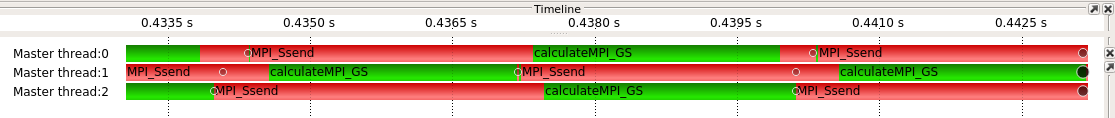
\includegraphics[width=14cm]{c_end_GS_3x2.png}
\end{figure}

\begin{figure}[h!]
 \caption{Endphase GS 3/2 (Patrick)}
 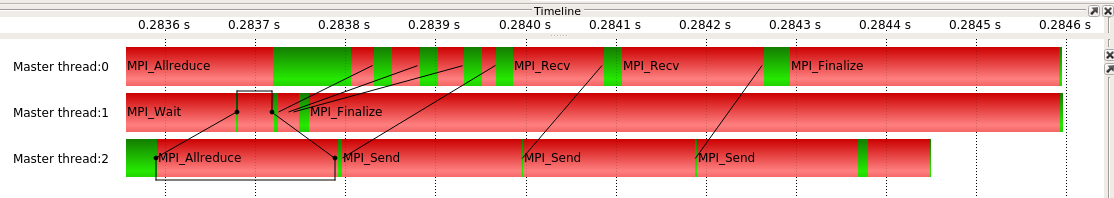
\includegraphics[width=14cm]{Patrick/c_end_GS_3x2.png}
\end{figure}
\begin{figure}[h!]
 \caption{Endphase GS 5/4 (Patrick)}
 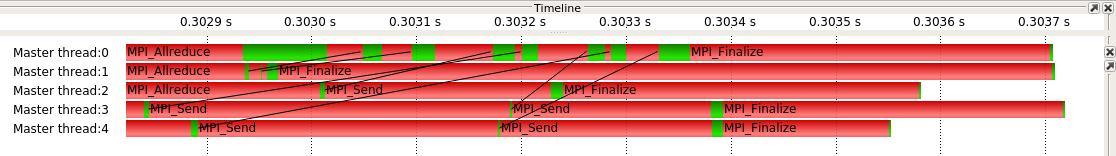
\includegraphics[width=14cm]{Patrick/c_end_GS_5x4.png}
\end{figure}
\begin{figure}[h!]
 \caption{Endphase JA 3/2}
 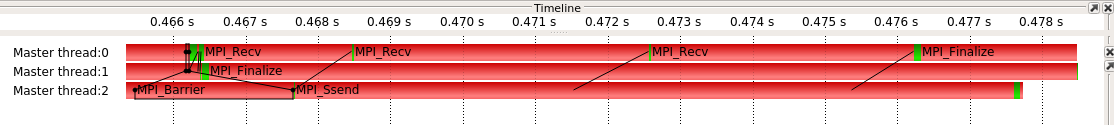
\includegraphics[width=14cm]{c_end_JA_3x2.png}
\end{figure}
\begin{figure}[h!]
 \caption{Endphase JA 3/2 (Patrick)}
 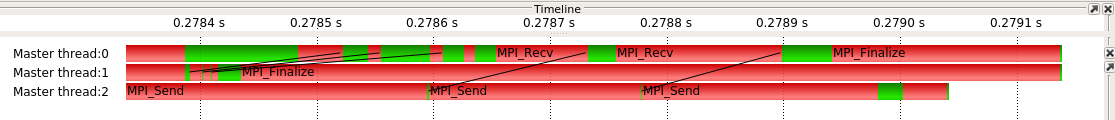
\includegraphics[width=14cm]{Patrick/c_end_JA_3x2.png}
\end{figure}
\begin{figure}[h!]
 \caption{Endphase JA 5/4 (Patrick)}
 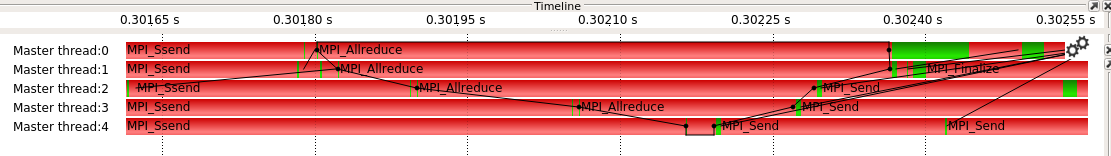
\includegraphics[width=14cm]{Patrick/c_end_JA_5x4.png}
\end{figure}
\end{document}
